\documentclass[twoside]{book}

% Packages required by doxygen
\usepackage{fixltx2e}
\usepackage{calc}
\usepackage{doxygen}
\usepackage[export]{adjustbox} % also loads graphicx
\usepackage{graphicx}
\usepackage[utf8]{inputenc}
\usepackage{makeidx}
\usepackage{multicol}
\usepackage{multirow}
\PassOptionsToPackage{warn}{textcomp}
\usepackage{textcomp}
\usepackage[nointegrals]{wasysym}
\usepackage[table]{xcolor}

% Font selection
\usepackage[T1]{fontenc}
\usepackage[scaled=.90]{helvet}
\usepackage{courier}
\usepackage{amssymb}
\usepackage{sectsty}
\renewcommand{\familydefault}{\sfdefault}
\allsectionsfont{%
  \fontseries{bc}\selectfont%
  \color{darkgray}%
}
\renewcommand{\DoxyLabelFont}{%
  \fontseries{bc}\selectfont%
  \color{darkgray}%
}
\newcommand{\+}{\discretionary{\mbox{\scriptsize$\hookleftarrow$}}{}{}}

% Page & text layout
\usepackage{geometry}
\geometry{%
  a4paper,%
  top=2.5cm,%
  bottom=2.5cm,%
  left=2.5cm,%
  right=2.5cm%
}
\tolerance=750
\hfuzz=15pt
\hbadness=750
\setlength{\emergencystretch}{15pt}
\setlength{\parindent}{0cm}
\setlength{\parskip}{3ex plus 2ex minus 2ex}
\makeatletter
\renewcommand{\paragraph}{%
  \@startsection{paragraph}{4}{0ex}{-1.0ex}{1.0ex}{%
    \normalfont\normalsize\bfseries\SS@parafont%
  }%
}
\renewcommand{\subparagraph}{%
  \@startsection{subparagraph}{5}{0ex}{-1.0ex}{1.0ex}{%
    \normalfont\normalsize\bfseries\SS@subparafont%
  }%
}
\makeatother

% Headers & footers
\usepackage{fancyhdr}
\pagestyle{fancyplain}
\fancyhead[LE]{\fancyplain{}{\bfseries\thepage}}
\fancyhead[CE]{\fancyplain{}{}}
\fancyhead[RE]{\fancyplain{}{\bfseries\leftmark}}
\fancyhead[LO]{\fancyplain{}{\bfseries\rightmark}}
\fancyhead[CO]{\fancyplain{}{}}
\fancyhead[RO]{\fancyplain{}{\bfseries\thepage}}
\fancyfoot[LE]{\fancyplain{}{}}
\fancyfoot[CE]{\fancyplain{}{}}
\fancyfoot[RE]{\fancyplain{}{\bfseries\scriptsize Generated by Doxygen }}
\fancyfoot[LO]{\fancyplain{}{\bfseries\scriptsize Generated by Doxygen }}
\fancyfoot[CO]{\fancyplain{}{}}
\fancyfoot[RO]{\fancyplain{}{}}
\renewcommand{\footrulewidth}{0.4pt}
\renewcommand{\chaptermark}[1]{%
  \markboth{#1}{}%
}
\renewcommand{\sectionmark}[1]{%
  \markright{\thesection\ #1}%
}

% Indices & bibliography
\usepackage{natbib}
\usepackage[titles]{tocloft}
\setcounter{tocdepth}{3}
\setcounter{secnumdepth}{5}
\makeindex

% Hyperlinks (required, but should be loaded last)
\usepackage{ifpdf}
\ifpdf
  \usepackage[pdftex,pagebackref=true]{hyperref}
\else
  \usepackage[ps2pdf,pagebackref=true]{hyperref}
\fi
\hypersetup{%
  colorlinks=true,%
  linkcolor=blue,%
  citecolor=blue,%
  unicode%
}

% Custom commands
\newcommand{\clearemptydoublepage}{%
  \newpage{\pagestyle{empty}\cleardoublepage}%
}

\usepackage{caption}
\captionsetup{labelsep=space,justification=centering,font={bf},singlelinecheck=off,skip=4pt,position=top}

%===== C O N T E N T S =====

\begin{document}

% Titlepage & ToC
\hypersetup{pageanchor=false,
             bookmarksnumbered=true,
             pdfencoding=unicode
            }
\pagenumbering{roman}
\begin{titlepage}
\vspace*{7cm}
\begin{center}%
{\Large My Project }\\
\vspace*{1cm}
{\large Generated by Doxygen 1.8.11}\\
\end{center}
\end{titlepage}
\clearemptydoublepage
\tableofcontents
\clearemptydoublepage
\pagenumbering{arabic}
\hypersetup{pageanchor=true}

%--- Begin generated contents ---
\chapter{Class Index}
\section{Class List}
Here are the classes, structs, unions and interfaces with brief descriptions\+:\begin{DoxyCompactList}
\item\contentsline{section}{\hyperlink{structnode}{node} }{\pageref{structnode}}{}
\item\contentsline{section}{\hyperlink{structnode1}{node1} }{\pageref{structnode1}}{}
\item\contentsline{section}{\hyperlink{structnode__info}{node\+\_\+info} }{\pageref{structnode__info}}{}
\end{DoxyCompactList}

\chapter{File Index}
\section{File List}
Here is a list of all files with brief descriptions\+:\begin{DoxyCompactList}
\item\contentsline{section}{\hyperlink{Lab1_8c}{Lab1.\+c} }{\pageref{Lab1_8c}}{}
\end{DoxyCompactList}

\chapter{Class Documentation}
\hypertarget{classGraph}{}\section{Graph Class Reference}
\label{classGraph}\index{Graph@{Graph}}
\subsection*{Public Member Functions}
\begin{DoxyCompactItemize}
\item 
\hyperlink{classGraph_af3ff6b295df8bf3bee0bafd7c7d56915}{Graph} (int \hyperlink{classGraph_a2b722f7cfa7a21e4cb5fae488b3d4dcc}{V})
\item 
\hyperlink{classGraph_a902c5b3eacb66d60752525ab23297a95}{$\sim$\+Graph} ()
\item 
void \hyperlink{classGraph_a8a3b5afce00f9d260b01c188fbe73f53}{add\+Edge} (int v, int w)
\item 
int \hyperlink{classGraph_a126588ac82d1075cb30972ead08daa94}{is\+Eulerian} ()
\item 
bool \hyperlink{classGraph_add6f4a13a70d1b15f370db0bd4669b90}{is\+Connected} ()
\item 
void \hyperlink{classGraph_a47d02784c897a7e0d42a29c698161648}{D\+F\+S\+Util} (int v, bool visited\mbox{[}$\,$\mbox{]})
\end{DoxyCompactItemize}
\subsection*{Private Attributes}
\begin{DoxyCompactItemize}
\item 
int \hyperlink{classGraph_a2b722f7cfa7a21e4cb5fae488b3d4dcc}{V}
\item 
list$<$ int $>$ $\ast$ \hyperlink{classGraph_a04ab9c17ad31aa036def8db0f88b035b}{adj}
\end{DoxyCompactItemize}


\subsection{Constructor \& Destructor Documentation}
\index{Graph@{Graph}!Graph@{Graph}}
\index{Graph@{Graph}!Graph@{Graph}}
\subsubsection[{\texorpdfstring{Graph(int V)}{Graph(int V)}}]{\setlength{\rightskip}{0pt plus 5cm}Graph\+::\+Graph (
\begin{DoxyParamCaption}
\item[{int}]{V}
\end{DoxyParamCaption}
)\hspace{0.3cm}{\ttfamily [inline]}}\hypertarget{classGraph_af3ff6b295df8bf3bee0bafd7c7d56915}{}\label{classGraph_af3ff6b295df8bf3bee0bafd7c7d56915}

\begin{DoxyCode}
14         \{
15             this->\hyperlink{classGraph_a2b722f7cfa7a21e4cb5fae488b3d4dcc}{V} = \hyperlink{classGraph_a2b722f7cfa7a21e4cb5fae488b3d4dcc}{V};
16             \hyperlink{classGraph_a04ab9c17ad31aa036def8db0f88b035b}{adj} = \textcolor{keyword}{new} list<int> [\hyperlink{classGraph_a2b722f7cfa7a21e4cb5fae488b3d4dcc}{V}];
17         \}
\end{DoxyCode}
\index{Graph@{Graph}!````~Graph@{$\sim$\+Graph}}
\index{````~Graph@{$\sim$\+Graph}!Graph@{Graph}}
\subsubsection[{\texorpdfstring{$\sim$\+Graph()}{~Graph()}}]{\setlength{\rightskip}{0pt plus 5cm}Graph\+::$\sim$\+Graph (
\begin{DoxyParamCaption}
{}
\end{DoxyParamCaption}
)\hspace{0.3cm}{\ttfamily [inline]}}\hypertarget{classGraph_a902c5b3eacb66d60752525ab23297a95}{}\label{classGraph_a902c5b3eacb66d60752525ab23297a95}

\begin{DoxyCode}
19         \{
20             \textcolor{keyword}{delete}[] \hyperlink{classGraph_a04ab9c17ad31aa036def8db0f88b035b}{adj};
21         \} \textcolor{comment}{// To avoid memory leak}
\end{DoxyCode}


\subsection{Member Function Documentation}
\index{Graph@{Graph}!add\+Edge@{add\+Edge}}
\index{add\+Edge@{add\+Edge}!Graph@{Graph}}
\subsubsection[{\texorpdfstring{add\+Edge(int v, int w)}{addEdge(int v, int w)}}]{\setlength{\rightskip}{0pt plus 5cm}void Graph\+::add\+Edge (
\begin{DoxyParamCaption}
\item[{int}]{v, }
\item[{int}]{w}
\end{DoxyParamCaption}
)}\hypertarget{classGraph_a8a3b5afce00f9d260b01c188fbe73f53}{}\label{classGraph_a8a3b5afce00f9d260b01c188fbe73f53}

\begin{DoxyCode}
37 \{
38     \hyperlink{classGraph_a04ab9c17ad31aa036def8db0f88b035b}{adj}[v].push\_back(w);
39     \hyperlink{classGraph_a04ab9c17ad31aa036def8db0f88b035b}{adj}[w].push\_back(v); \textcolor{comment}{// Note: the graph is undirected}
40 \}
\end{DoxyCode}
\index{Graph@{Graph}!D\+F\+S\+Util@{D\+F\+S\+Util}}
\index{D\+F\+S\+Util@{D\+F\+S\+Util}!Graph@{Graph}}
\subsubsection[{\texorpdfstring{D\+F\+S\+Util(int v, bool visited[])}{DFSUtil(int v, bool visited[])}}]{\setlength{\rightskip}{0pt plus 5cm}void Graph\+::\+D\+F\+S\+Util (
\begin{DoxyParamCaption}
\item[{int}]{v, }
\item[{bool}]{visited\mbox{[}$\,$\mbox{]}}
\end{DoxyParamCaption}
)}\hypertarget{classGraph_a47d02784c897a7e0d42a29c698161648}{}\label{classGraph_a47d02784c897a7e0d42a29c698161648}

\begin{DoxyCode}
43 \{
44     \textcolor{comment}{// Mark the current node as visited and print it}
45     visited[v] = \textcolor{keyword}{true};
46  
47     \textcolor{comment}{// Recur for all the vertices adjacent to this vertex}
48     list<int>::iterator i;
49     \textcolor{keywordflow}{for} (i = \hyperlink{classGraph_a04ab9c17ad31aa036def8db0f88b035b}{adj}[v].begin(); i != \hyperlink{classGraph_a04ab9c17ad31aa036def8db0f88b035b}{adj}[v].end(); ++i)
50         \textcolor{keywordflow}{if} (!visited[*i])
51             \hyperlink{classGraph_a47d02784c897a7e0d42a29c698161648}{DFSUtil}(*i, visited);
52 \}
\end{DoxyCode}
\index{Graph@{Graph}!is\+Connected@{is\+Connected}}
\index{is\+Connected@{is\+Connected}!Graph@{Graph}}
\subsubsection[{\texorpdfstring{is\+Connected()}{isConnected()}}]{\setlength{\rightskip}{0pt plus 5cm}bool Graph\+::is\+Connected (
\begin{DoxyParamCaption}
{}
\end{DoxyParamCaption}
)}\hypertarget{classGraph_add6f4a13a70d1b15f370db0bd4669b90}{}\label{classGraph_add6f4a13a70d1b15f370db0bd4669b90}

\begin{DoxyCode}
57 \{
58     \textcolor{comment}{// Mark all the vertices as not visited}
59     \textcolor{keywordtype}{bool} visited[\hyperlink{classGraph_a2b722f7cfa7a21e4cb5fae488b3d4dcc}{V}];
60     \textcolor{keywordtype}{int} i;
61     \textcolor{keywordflow}{for} (i = 0; i < \hyperlink{classGraph_a2b722f7cfa7a21e4cb5fae488b3d4dcc}{V}; i++)
62         visited[i] = \textcolor{keyword}{false};
63  
64     \textcolor{comment}{// Find a vertex with non-zero degree}
65     \textcolor{keywordflow}{for} (i = 0; i < \hyperlink{classGraph_a2b722f7cfa7a21e4cb5fae488b3d4dcc}{V}; i++)
66         \textcolor{keywordflow}{if} (\hyperlink{classGraph_a04ab9c17ad31aa036def8db0f88b035b}{adj}[i].size() != 0)
67             \textcolor{keywordflow}{break};
68  
69     \textcolor{comment}{// If there are no edges in the graph, return true}
70     \textcolor{keywordflow}{if} (i == V)
71         \textcolor{keywordflow}{return} \textcolor{keyword}{true};
72  
73     \textcolor{comment}{// Start DFS traversal from a vertex with non-zero degree}
74     \hyperlink{classGraph_a47d02784c897a7e0d42a29c698161648}{DFSUtil}(i, visited);
75  
76     \textcolor{comment}{// Check if all non-zero degree vertices are visited}
77     \textcolor{keywordflow}{for} (i = 0; i < \hyperlink{classGraph_a2b722f7cfa7a21e4cb5fae488b3d4dcc}{V}; i++)
78         \textcolor{keywordflow}{if} (visited[i] == \textcolor{keyword}{false} && \hyperlink{classGraph_a04ab9c17ad31aa036def8db0f88b035b}{adj}[i].size() > 0)
79             \textcolor{keywordflow}{return} \textcolor{keyword}{false};
80  
81     \textcolor{keywordflow}{return} \textcolor{keyword}{true};
82 \}
\end{DoxyCode}
\index{Graph@{Graph}!is\+Eulerian@{is\+Eulerian}}
\index{is\+Eulerian@{is\+Eulerian}!Graph@{Graph}}
\subsubsection[{\texorpdfstring{is\+Eulerian()}{isEulerian()}}]{\setlength{\rightskip}{0pt plus 5cm}int Graph\+::is\+Eulerian (
\begin{DoxyParamCaption}
{}
\end{DoxyParamCaption}
)}\hypertarget{classGraph_a126588ac82d1075cb30972ead08daa94}{}\label{classGraph_a126588ac82d1075cb30972ead08daa94}

\begin{DoxyCode}
89 \{
90     \textcolor{comment}{// Check if all non-zero degree vertices are connected}
91     \textcolor{keywordflow}{if} (\hyperlink{classGraph_add6f4a13a70d1b15f370db0bd4669b90}{isConnected}() == \textcolor{keyword}{false})
92         \textcolor{keywordflow}{return} 0;
93  
94     \textcolor{comment}{// Count vertices with odd degree}
95     \textcolor{keywordtype}{int} odd = 0;
96     \textcolor{keywordflow}{for} (\textcolor{keywordtype}{int} i = 0; i < \hyperlink{classGraph_a2b722f7cfa7a21e4cb5fae488b3d4dcc}{V}; i++)
97         \textcolor{keywordflow}{if} (\hyperlink{classGraph_a04ab9c17ad31aa036def8db0f88b035b}{adj}[i].size() & 1)
98             odd++;
99  
100     \textcolor{comment}{// If count is more than 2, then graph is not Eulerian}
101     \textcolor{keywordflow}{if} (odd > 2)
102         \textcolor{keywordflow}{return} 0;
103  
104     \textcolor{comment}{// If odd count is 2, then semi-eulerian.}
105     \textcolor{comment}{// If odd count is 0, then eulerian}
106     \textcolor{comment}{// Note that odd count can never be 1 for undirected graph}
107     \textcolor{keywordflow}{return} (odd) ? 1 : 2;
108 \}
\end{DoxyCode}


\subsection{Member Data Documentation}
\index{Graph@{Graph}!adj@{adj}}
\index{adj@{adj}!Graph@{Graph}}
\subsubsection[{\texorpdfstring{adj}{adj}}]{\setlength{\rightskip}{0pt plus 5cm}list$<$int$>$$\ast$ Graph\+::adj\hspace{0.3cm}{\ttfamily [private]}}\hypertarget{classGraph_a04ab9c17ad31aa036def8db0f88b035b}{}\label{classGraph_a04ab9c17ad31aa036def8db0f88b035b}
\index{Graph@{Graph}!V@{V}}
\index{V@{V}!Graph@{Graph}}
\subsubsection[{\texorpdfstring{V}{V}}]{\setlength{\rightskip}{0pt plus 5cm}int Graph\+::V\hspace{0.3cm}{\ttfamily [private]}}\hypertarget{classGraph_a2b722f7cfa7a21e4cb5fae488b3d4dcc}{}\label{classGraph_a2b722f7cfa7a21e4cb5fae488b3d4dcc}


The documentation for this class was generated from the following file\+:\begin{DoxyCompactItemize}
\item 
\hyperlink{EulerianCycle_8cpp}{Eulerian\+Cycle.\+cpp}\end{DoxyCompactItemize}

\chapter{File Documentation}
\hypertarget{DirectedGraph_8cpp}{}\section{Directed\+Graph.\+cpp File Reference}
\label{DirectedGraph_8cpp}\index{Directed\+Graph.\+cpp@{Directed\+Graph.\+cpp}}
{\ttfamily \#include $<$iostream$>$}\\*
{\ttfamily \#include $<$list$>$}\\*
{\ttfamily \#include $<$stack$>$}\\*
Include dependency graph for Directed\+Graph.\+cpp\+:
\nopagebreak
\begin{figure}[H]
\begin{center}
\leavevmode
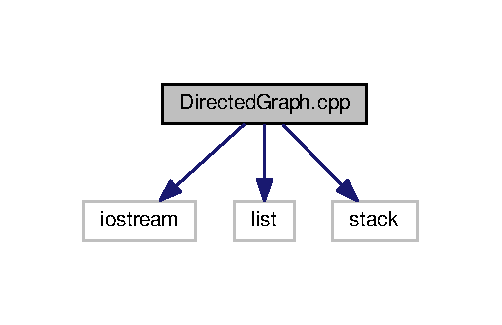
\includegraphics[width=241pt]{DirectedGraph_8cpp__incl}
\end{center}
\end{figure}
\subsection*{Classes}
\begin{DoxyCompactItemize}
\item 
class \hyperlink{classGraph}{Graph}
\end{DoxyCompactItemize}
\subsection*{Functions}
\begin{DoxyCompactItemize}
\item 
int \hyperlink{DirectedGraph_8cpp_ae66f6b31b5ad750f1fe042a706a4e3d4}{main} ()
\end{DoxyCompactItemize}


\subsection{Function Documentation}
\index{Directed\+Graph.\+cpp@{Directed\+Graph.\+cpp}!main@{main}}
\index{main@{main}!Directed\+Graph.\+cpp@{Directed\+Graph.\+cpp}}
\subsubsection[{\texorpdfstring{main()}{main()}}]{\setlength{\rightskip}{0pt plus 5cm}int main (
\begin{DoxyParamCaption}
{}
\end{DoxyParamCaption}
)}\hypertarget{DirectedGraph_8cpp_ae66f6b31b5ad750f1fe042a706a4e3d4}{}\label{DirectedGraph_8cpp_ae66f6b31b5ad750f1fe042a706a4e3d4}

\begin{DoxyCode}
109 \{
110     \textcolor{comment}{// Create graphs given in the above diagrams}
111     \hyperlink{classGraph}{Graph} g1(5);
112     g1.addEdge(0, 1);
113     g1.addEdge(1, 2);
114     g1.addEdge(2, 3);
115     g1.addEdge(3, 0);
116     g1.addEdge(2, 4);
117     g1.addEdge(4, 2);
118     cout << \textcolor{stringliteral}{"The graph is weakly connected? "};
119     g1.isSC() ? cout << \textcolor{stringliteral}{"No\(\backslash\)n"} : cout << \textcolor{stringliteral}{"Yes\(\backslash\)n"};
120  
121     \hyperlink{classGraph}{Graph} g2(4);
122     g2.addEdge(0, 1);
123     g2.addEdge(1, 2);
124     g2.addEdge(2, 3);
125     cout << \textcolor{stringliteral}{"The graph is weakly connected? "};
126     g2.isSC() ? cout << \textcolor{stringliteral}{"No\(\backslash\)n"} : cout << \textcolor{stringliteral}{"Yes\(\backslash\)n"};
127  
128     \textcolor{keywordflow}{return} 0;
129 \}\end{DoxyCode}


Here is the call graph for this function\+:
\nopagebreak
\begin{figure}[H]
\begin{center}
\leavevmode
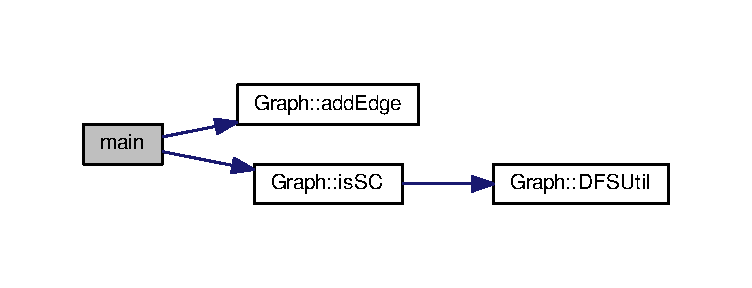
\includegraphics[width=350pt]{DirectedGraph_8cpp_ae66f6b31b5ad750f1fe042a706a4e3d4_cgraph}
\end{center}
\end{figure}



%--- End generated contents ---

% Index
\backmatter
\newpage
\phantomsection
\clearemptydoublepage
\addcontentsline{toc}{chapter}{Index}
\printindex

\end{document}
